% =====================================================================================
%  SvaraMitra -- IEEE Transactions template (IEEEtran, journal mode)
%
%  OVERLEAF
%   - Upload main.tex and the figures/ folder (or upload the zip as a new project).
%     figures/ must contain: fig_task_conflict.png, fig1_svaramitra_pipeline.png,
%     fig_train_vs_infer.png, fig_task_depth.png
%     References are inline (thebibliography); no .bib file is needed.
%   - Compiler: pdfLaTeX. IEEEtran.cls is built into Overleaf.
%   - Red text = items only the authors can supply (or results still being measured). Search for "\ph{" to find them.
% =====================================================================================
\documentclass[lettersize,journal]{IEEEtran}

\usepackage{amsmath,amsfonts,amssymb}
\usepackage{array}
\usepackage{textcomp}
\usepackage{stfloats}
\usepackage{url}
\usepackage{graphicx}
\usepackage{cite}
\usepackage{xcolor}
\usepackage{booktabs}
\usepackage{multirow}
\usepackage[plain]{algorithm}
\usepackage{algorithmic}
\usepackage[hidelinks]{hyperref}

\hyphenation{op-tical net-works semi-conduc-tor Zip-former Vox-Celeb Libri-Speech}

% ---------- helpers ----------
\newcommand{\ph}[1]{\textcolor{red}{[#1]}}          % item only the authors can supply / result still pending
\newcommand{\method}{SvaraMitra}                    % change here to rename the method everywhere
\newcolumntype{L}[1]{>{\raggedright\arraybackslash}p{#1}}
\renewcommand{\algorithmicrequire}{\textbf{Require:}}
\renewcommand{\algorithmicensure}{\textbf{Ensure:}}

\begin{document}

\title{SvaraMitra: A Lightweight Multi-Task Audio Intelligence Framework for Speech Recognition, Audio Event Detection, and Speaker Verification}

% Author grid (2 rows x 3 authors): name / department / institution / city / e-mail
\newcommand{\authorcell}[5]{%
  \begin{tabular}[t]{@{}>{\centering\arraybackslash}p{0.30\textwidth}@{}}
    #1\\ \textit{#2}\\ \textit{#3}\\ #4\\ #5
  \end{tabular}}
\author{%
\begin{tabular}{@{}ccc@{}}
  \authorcell{P.~V.~N.~Balram~Murthy}{Department of Computer Science and Engineering}{Neil Gogte Institute of Technology}{Hyderabad, India}{balaram@kmit.in} &
  \authorcell{R.~Vanusshka}{Department of Computer Science and Engineering}{Keshav Memorial Engineering College}{Hyderabad, India}{ravurivanusshka@gmail.com} &
  \authorcell{U.~Prashanth}{Department of Computer Science and Engineering}{Keshav Memorial Engineering College}{Hyderabad, India}{uprashanth222@gmail.com} \\[1.5em]
  \authorcell{P.~Mohammad~Mansur}{Department of Computer Science and Engineering}{Keshav Memorial Engineering College}{Hyderabad, India}{mohammadmansurpolikimulla@\allowbreak gmail.com} &
  \authorcell{B.~Pavithra}{Department of Computer Science and Engineering}{Keshav Memorial Engineering College}{Hyderabad, India}{bokkalapavithra22@gmail.com} &
  \authorcell{Nithyantha}{Department of Computer Science and Engineering}{Keshav Memorial Engineering College}{Hyderabad, India}{mnithya@gmail.com}
\end{tabular}}

\maketitle
% no running header, page numbers or first-page footer
\pagestyle{empty}
\thispagestyle{empty}

% ================================================================ ABSTRACT
\begin{abstract}
A single audio encoder that handles speech recognition (ASR), audio tagging (AT), and speaker verification (SV)
would save parameters and computation, but the three tasks differ in labels, input representations, and training
objectives, which makes joint training hard. MT2KD~\cite{yang2025mt2kd} tackled this with multi-teacher knowledge
distillation followed by supervised fine-tuning. We present \method{}, a multi-task audio framework that follows
this two-stage recipe and makes two changes. First, we replace the original teachers with three smaller specialist
models, WavLM-Large for speech, SSLAM for sound events, and ReDimNet2-B6 for speakers, which cuts the teacher
parameters from about 750M to about 418M; each replacement was chosen by a controlled comparison. Second, we add a
compact 22M Zipformer-S student that learns from the three teachers and from our trained 64M Zipformer-M model,
used as a frozen teaching assistant, with the layers that both encoders share copied from the 64M model. Trained on
a small budget of 30 hours of speech, 15,000 sound clips, and 1,171 speakers, with the same data and schedule for
both models, the 22M student reaches 43.36\% WER on LibriSpeech test-clean with greedy CTC, 43.07\% mAP on FSD50K,
and 4.30\% EER on VoxCeleb1-O, against 45.08\%, 39.36\%, and 8.44\% for the 64M model, while being 2.9$\times$
smaller and 1.46$\times$ faster on a CPU. The student is also far more stable when the encoder is unfrozen during
fine-tuning. A word-level 3-gram language model, tested as a separate decoding condition, lowers the dev-clean WER
of the 64M model from 46.33\% to 20.42\%. A CPU web application demonstrates all three tasks with one model.
\end{abstract}

\begin{IEEEkeywords}
Multi-task audio learning, knowledge distillation, multi-teacher distillation, teaching-assistant distillation,
Zipformer, speech recognition, audio tagging, speaker verification.
\end{IEEEkeywords}

% ================================================================ I. INTRODUCTION
\section{Introduction}
\IEEEPARstart{E}{nd-to-end} models now perform very well on speech recognition, sound-event tagging, and speaker
verification, but each is usually built separately, with its own architecture, features, and data. A single shared
encoder would save parameters and computation, and could also serve as the audio front end of speech-based large
language models.

\textit{Why it is hard.} The tasks prefer different inputs (frame-level features for ASR and SV, time--frequency
patches for strong taggers), draw on different corpora, and partly pull in opposite directions
(Fig.~\ref{fig:conflict}): ASR should ignore who is speaking, SV should ignore what is said, and AT needs every sound
event present, speech included. A multi-task model trained from scratch is therefore often worse on each task than a
dedicated model.

\begin{figure}[!htbp]
  \centering
  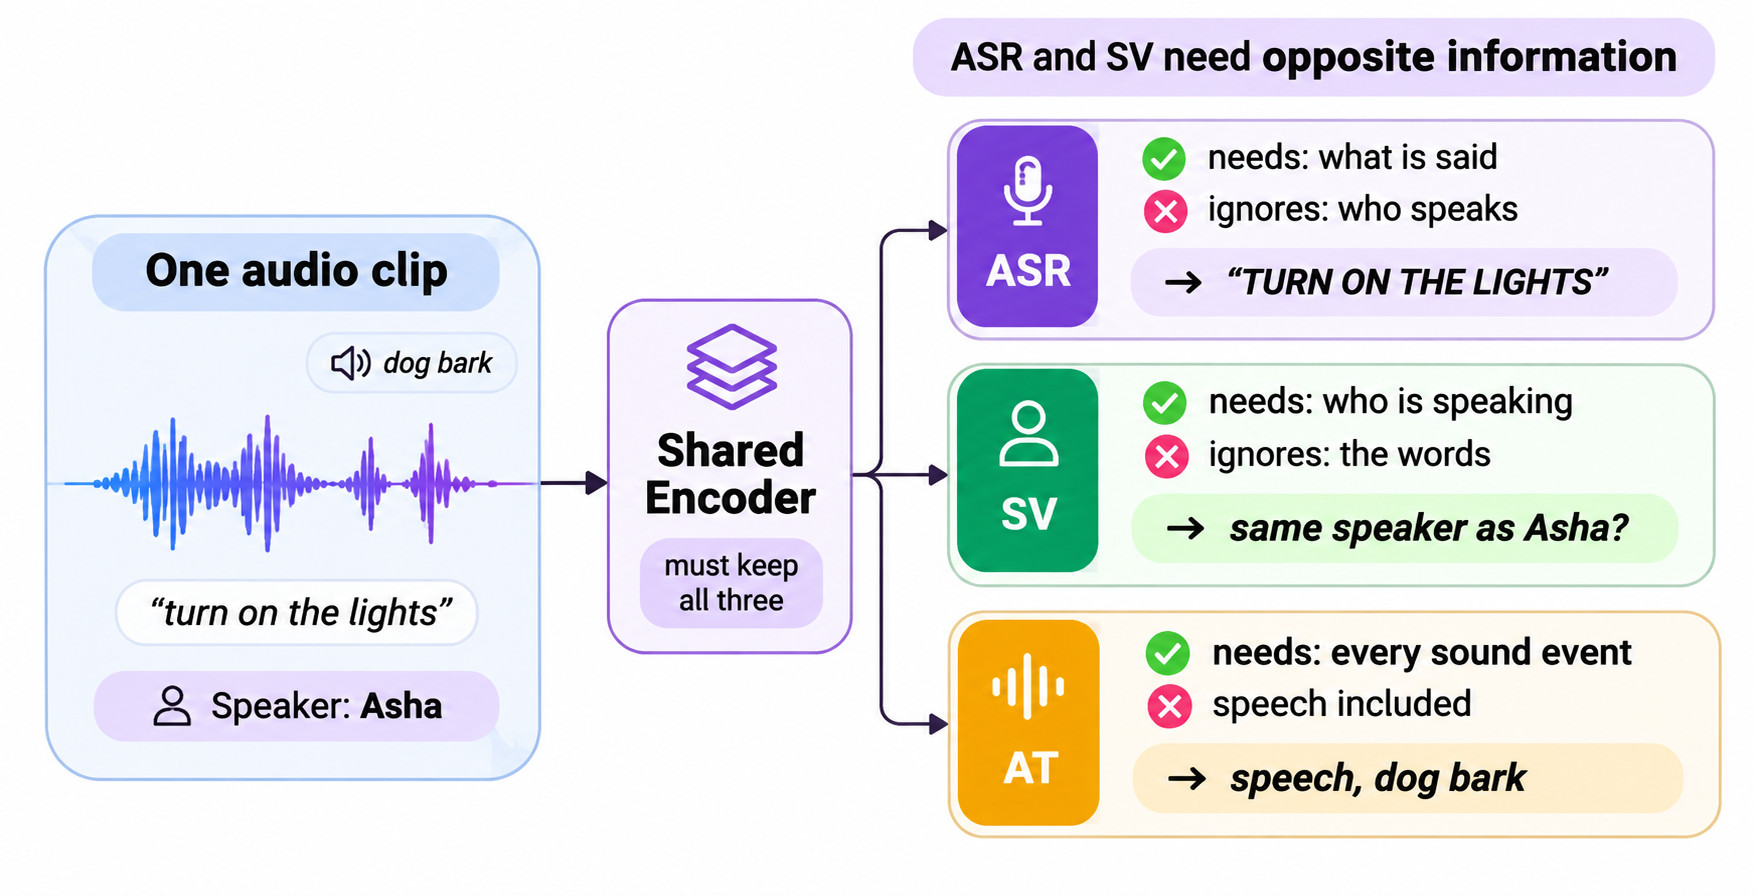
\includegraphics[width=\linewidth]{figures/fig_task_conflict.png}
  \caption{The three tasks read different information from the same audio clip. ASR needs what is said and should
  ignore the speaker, SV needs who is speaking and should ignore the words, and AT needs which sounds are present. A
  single shared encoder must keep all three.}
  \label{fig:conflict}
\end{figure}

\textit{Base work.} MT2KD~\cite{yang2025mt2kd} trains one Zipformer student in two stages: it first reproduces the
outputs of three frozen teachers (Whisper large-v3, BEATs, and ECAPA-TDNN) on unlabelled audio, with each task
attached at a different encoder depth, and is then fine-tuned on labelled data. Its 66\,M model comes close to the
best single-task systems.

\textit{Motivation and gap.} MT2KD relies on large teachers, most notably the 637\,M-parameter Whisper large-v3
encoder, and on training corpora far larger than a single-GPU budget allows. Running the teachers over the training
data is a large part of the training cost, and it is not obvious that the largest available teacher is the most
useful one for a small student. The student itself, at 66\,M parameters, is also larger than needed for many
on-device uses. We ask whether smaller specialist teachers can supervise the shared encoder at least as well, and
whether a much smaller encoder can match the 64\,M one when it is trained and deployed with modest resources.

\textit{Contributions.} \method{} keeps the shared-encoder idea and the two-stage recipe of MT2KD and contributes:
\begin{itemize}
  \item a replacement teacher set (WavLM-Large, SSLAM, ReDimNet2-B6) about 44\% smaller than MT2KD's (418\,M vs
  750\,M parameters), with measured evidence for each replacement;
  \item a complete two-stage implementation with a 64\,M Zipformer-M encoder on a small data budget, evaluated on
  LibriSpeech test-clean, FSD50K, and VoxCeleb1-O;
  \item a 22\,M Zipformer-S student trained with the 64\,M model as a frozen teaching assistant and with the shared
  stacks copied from it, which is 2.9$\times$ smaller, 1.46$\times$ faster, and better on all three tasks;
  \item a stage-wise analysis showing that fine-tuning degrades speaker verification and that the teaching assistant
  makes it far more stable, plus a CTC decoder with a 3-gram language model and a CPU web application.
\end{itemize}

The rest of the paper is organised as follows. Section~\ref{sec:related} reviews related work,
Section~\ref{sec:method} presents the proposed work, Section~\ref{sec:setup} describes the data and experiments,
Section~\ref{sec:results} gives the results, Section~\ref{sec:discussion} discusses limitations and ethics, and
Section~\ref{sec:conclusion} concludes.

% ================================================================ II. RELATED WORK
\section{Related Work}\label{sec:related}

\textit{Task-specific models.} End-to-end ASR pairs an acoustic encoder with CTC~\cite{graves2006ctc} or a neural
transducer~\cite{graves2012transducer}; large weakly supervised training, as in Whisper~\cite{radford2023whisper},
improved accuracy and robustness. Audio tagging moved from convolutional networks~\cite{choi2016tagging,kong2020panns}
to transformers on spectrogram patches, such as AST~\cite{gong2021ast} and BEATs~\cite{chen2023beats}. Speaker
verification compares embeddings such as x-vectors~\cite{snyder2019xvector} or ECAPA-TDNN~\cite{desplanques2020ecapa}
by cosine similarity.

\textit{Multi-task and general-purpose audio models.} Multi-task learning for speech has a long
history~\cite{tang2016multitask,pironkov2016overview}, and self-supervised models such as HuBERT~\cite{hsu2021hubert}
and WavLM~\cite{chen2022wavlm} serve many speech tasks~\cite{yang2021superb}; an encoder trained on many audio tasks
has also served as the audio branch of a language-supervised model~\cite{elizalde2024clap}. Combining speech and
non-speech tasks is less explored: Whisper-AT~\cite{gong2023whisperat} found that fine-tuning Whisper's encoder for
tagging conflicts with keeping its recognition accuracy.

\textit{Knowledge distillation.} A student learns to reproduce a teacher's outputs~\cite{hinton2014distilling,li2014smalldnn},
with targets computed offline or online~\cite{beyer2022patient}. It has been applied to CTC~\cite{takashima2018ctckd}
and transducer ASR~\cite{yang2022transducerkd}, to compress Whisper~\cite{gandhi2023distilwhisper}, to audio
tagging~\cite{schmid2023efficientat,dinkel2024ced}, and to speaker embeddings~\cite{wang2019speakerkd}. Several
teachers can pass on complementary knowledge~\cite{huang2023ensemblekd,yang2023multifoundation,ranzinger2024amradio},
and when the teacher--student gap is large, an intermediate \emph{teaching assistant} can bridge it~\cite{mirzadeh2020takd}.

\textit{Positioning.} MT2KD~\cite{yang2025mt2kd} distils an ASR, an AT, and an SV teacher into one Zipformer
student~\cite{yao2024zipformer}. We keep this framework and study two questions: the choice of teachers, replacing each
with a smaller specialist (WavLM~\cite{chen2022wavlm}, SSLAM~\cite{sslam}, ReDimNet2~\cite{redimnet2}), and the size of
the student, adding a teaching-assistant stage~\cite{mirzadeh2020takd} that compresses the 64\,M encoder into a 22\,M
one. Our work is an empirical study of established distillation ideas under a limited budget, not a new distillation
principle.

% ================================================================ III. PROPOSED WORK
\section{Proposed Work: \method{}}\label{sec:method}

% The architecture diagram belongs to the Proposed Work section. A full-width figure in IEEE two-column layout
% always appears at the top of a page, so it lands at the top of the first page after this heading.
\begin{figure*}[!t]
  \centering
  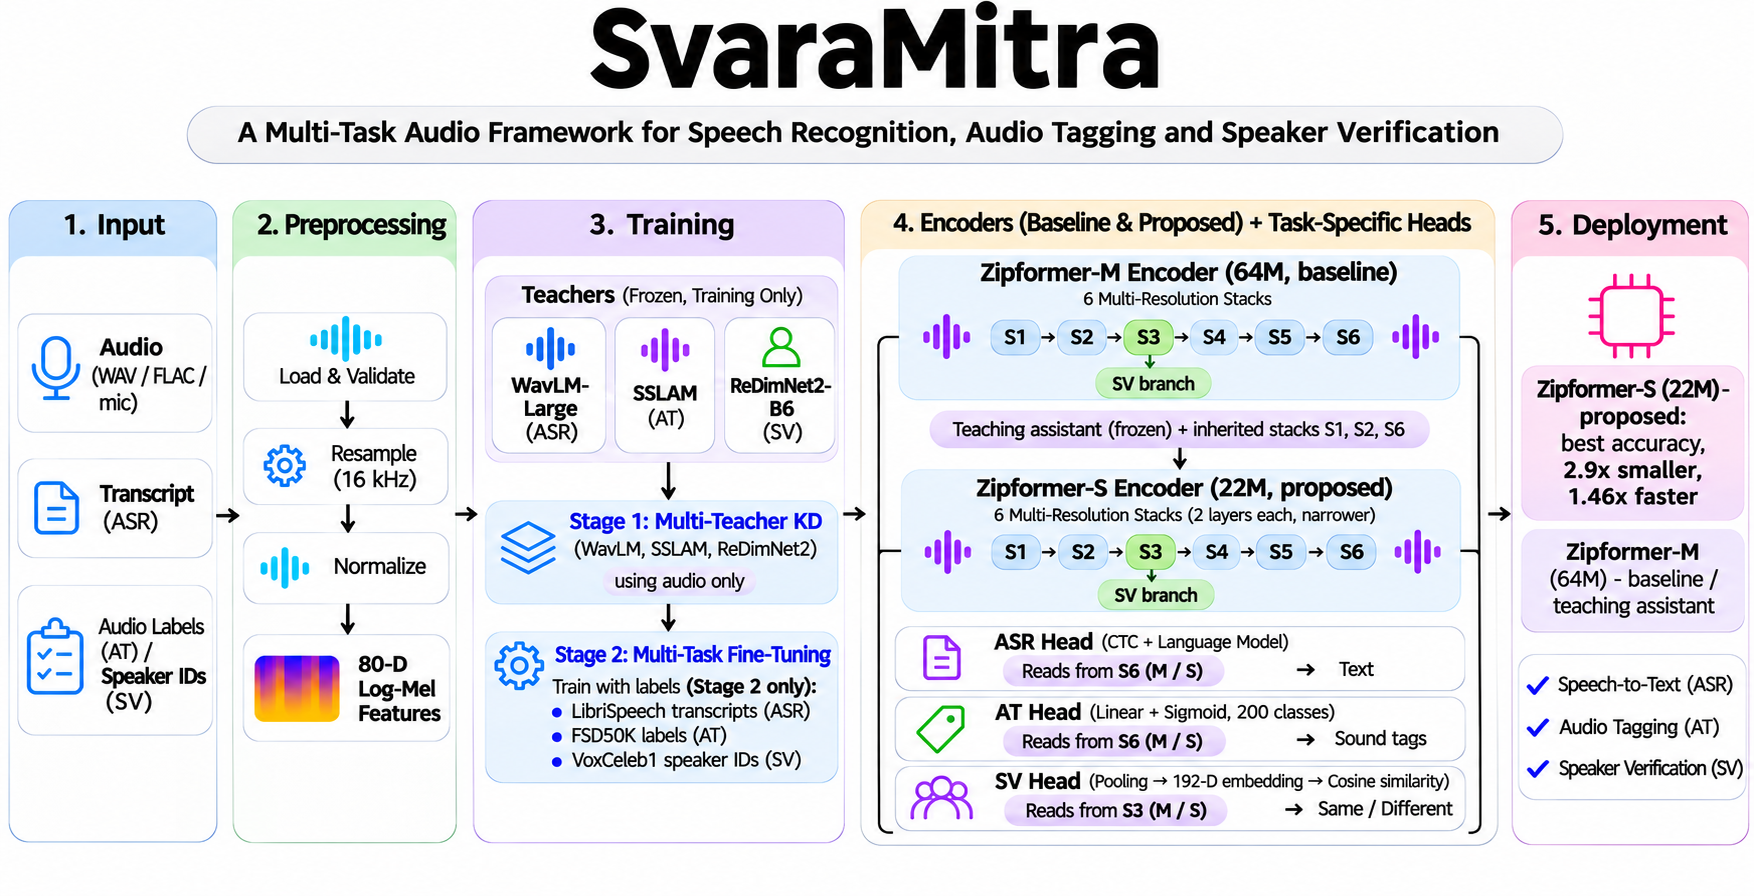
\includegraphics[width=\textwidth]{figures/fig1_svaramitra_pipeline.png}
  \caption{The \method{} multi-task pipeline: (1) audio with task labels, (2) preprocessing to 80-D log-Mel features,
  (3) Stage~1 multi-teacher distillation from frozen WavLM-Large, SSLAM, and ReDimNet2-B6 using audio only, followed
  by Stage~2 multi-task fine-tuning, (4) the two encoders, each with six stacks S1--S6: the 64\,M Zipformer-M
  (baseline) and the 22\,M Zipformer-S (proposed), which learns from the frozen Zipformer-M as a teaching assistant
  and inherits stacks S1, S2, and S6 from it; in both, the ASR and AT heads read from S6 and the SV head from S3, and
  (5) deployment of one model for three tasks. Teachers and the teaching assistant are used only in training.}
  \label{fig:pipeline}
\end{figure*}

\subsection{Overview and Problem Formulation}
Fig.~\ref{fig:pipeline} shows the pipeline. Audio is validated, converted to mono 16-kHz, and turned into 80-bin
log-Mel features $F(x)$ for the encoder, while each teacher receives the input its own checkpoint expects (for WavLM,
a per-utterance normalised waveform). In Stage~1 the encoder learns from three frozen teachers using audio only; in
Stage~2 it is fine-tuned with LibriSpeech transcripts, FSD50K labels, and VoxCeleb1 speaker IDs. Separate per-task
manifests keep the official test sets out of training and out of the teacher targets. The teachers, and for
Zipformer-S the teaching assistant, are used only in training; the deployed system is the encoder with its three
heads.

The encoder $E$ produces stack outputs $\mathbf{H}^{(3)}$ and $\mathbf{H}^{(6)}\in\mathbb{R}^{T'\times d}$, where
$\mathbf{H}^{(6)}$ is the final output at 25 frames per second ($d=512$ for Zipformer-M, $256$ for Zipformer-S). The
heads produce CTC character posteriors and 200 event probabilities from $\mathbf{H}^{(6)}$, and a 192-D speaker
embedding $\mathbf{e}(x)$ from $\mathbf{H}^{(3)}$; verification compares two normalised embeddings by cosine similarity.

\subsection{Specialist Teachers}\label{sec:teachers}
\textit{Why the teachers differ from MT2KD.} MT2KD~\cite{yang2025mt2kd} used Whisper large-v3, BEATs, and ECAPA-TDNN
as teachers. We replaced each with a model of smaller or equal size that measured better in our tests.
Table~\ref{tab:teacher_size} lists the replacements and their sizes: together they reduce the teacher parameters
that must be run during preprocessing and training from about 750\,M to about 418\,M, a 44\% reduction.

\begin{table}[!htbp]
  \caption{Teacher models: MT2KD versus ours}
  \label{tab:teacher_size}
  \centering
  \footnotesize
  \setlength{\tabcolsep}{3pt}
  \setlength{\tabcolsep}{2pt}
  \begin{tabular}{lL{2.0cm}cL{1.8cm}c}
    \toprule
    Task & MT2KD teacher & Params & Our teacher & Params \\
    \midrule
    ASR & Whisper-large-v3 (encoder only)$^{*}$ & 637M & \textbf{WavLM-Large} & 315M \\
    AT  & BEATs (AS2M) & 90.7M & \textbf{SSLAM} & 90.4M \\
    SV  & ECAPA-TDNN & $\sim$20.8M$^{\dagger}$ & \textbf{ReDimNet2-B6} & 12.3M \\
    \midrule
    Total & & $\sim$750M & & \textbf{$\sim$418M} \\
    & & & & \textbf{($-$44\%)} \\
    \bottomrule
    \multicolumn{5}{L{8.2cm}}{\scriptsize $^{*}$The full Whisper-large-v3 model has 1.55\,B parameters; only its encoder is used as the distillation teacher. $^{\dagger}$Approximate size of the public SpeechBrain ECAPA-TDNN VoxCeleb checkpoint.}
  \end{tabular}
\end{table}

Table~\ref{tab:teachers} gives the measurement behind each replacement.

\begin{table}[!htbp]
  \caption{Why each teacher was replaced: controlled comparisons}
  \label{tab:teachers}
  \centering
  \footnotesize
  \setlength{\tabcolsep}{3pt}
  \begin{tabular}{lL{3.3cm}L{1.45cm}L{1.95cm}}
    \toprule
    Task & Test & Original & Ours \\
    \midrule
    ASR & Same student, 2\,h distillation, frozen-encoder CTC probe, dev-clean WER $\downarrow$ & 81.93\% (Whisper) & \textbf{64.93\%} (WavLM) \\
    AT  & Teacher mAP on FSD50K val, 192 mapped classes $\uparrow$ & 50.29\% (BEATs) & \textbf{55.19\%} ($+$4.83; 95\% CI [$+$3.98, $+$5.76]) \\
    SV  & Teacher EER on VoxCeleb1-O $\downarrow$ & 11.16\% (WavLM, rejected) & \textbf{0.408\%} (ReDimNet2-B6) \\
    \bottomrule
  \end{tabular}
\end{table}

The ASR row compares students: the same 64\,M Zipformer-M was distilled for 30 epochs on 2\,h of train-clean-100
from each teacher, frozen, and probed with a two-layer BiLSTM CTC model trained on 10\,h of transcribed speech; a
student with no teacher reached 86.59\%. The AT row compares the teachers themselves on the 4,170 FSD50K validation
clips, with a paired-bootstrap confidence interval. The SV row reports the teacher's own EER; a frozen WavLM-Large,
first tried as the SV teacher, gave 11.16\% and was rejected. The probe WERs come from a separate experiment and are
not comparable with those in Section~\ref{sec:results}.

\textit{Teacher details.} WavLM is a representation teacher: its 1024-D, 50-Hz layer-24 frames are paired into
2048-D targets at the encoder's 25\,Hz, the alignment is measured on real utterances, padded frames are masked, and a
linear projection maps the encoder output to the target space. SSLAM's 527 AudioSet outputs are matched to FSD50K by
AudioSet identifier rather than output index, because the public BEATs checkpoint does not use the standard class
order; 192 of the 200 FSD50K classes have a counterpart, which also initialise the Stage-2 AT head. For SV, teacher and
encoder see the same centred crop of at most 20\,s, and the raw ReDimNet2-B6 embedding is the target (0.870\% EER on
20,000 held-out trials, vs 0.880\% centred and 0.920\% standardised).

\subsection{Encoder Architectures and Task Heads}
The baseline encoder is the Zipformer-M configuration of the Icefall toolkit~\cite{yao2024zipformer}: a convolutional
subsampling front end followed by six stacks with 2, 2, 3, 4, 3, and 2 layers, embedding dimensions of 192, 256,
384, 512, 384, and 256, feed-forward dimensions of 512, 768, 1,024, 1,536, 1,024, and 768, and 4, 4, 4, 8, 4, and 4
attention heads. The stacks run at downsampling factors of 1, 2, 4, 8, 4, and 2 relative to the subsampled frame
rate, and the final output runs at 25 frames per second. The encoder has 63.99\,M parameters and the task heads add
0.36\,M. The proposed Zipformer-S follows the ``S'' configuration of the Zipformer paper~\cite{yao2024zipformer}:
the same front end, six stacks, downsampling factors, and attention heads, but with two layers in every stack and
narrower middle stacks. Table~\ref{tab:zipcfg} compares the two.

\begin{table}[!htbp]
  \caption{The two encoder configurations (stacks S1--S6)}
  \label{tab:zipcfg}
  \centering
  \footnotesize
  \setlength{\tabcolsep}{3pt}
  \begin{tabular}{L{2.2cm}L{2.75cm}L{2.75cm}}
    \toprule
    & Zipformer-M (baseline) & Zipformer-S (proposed) \\
    \midrule
    Layers per stack      & 2, 2, 3, 4, 3, 2 & 2, 2, 2, 2, 2, 2 \\
    Embedding dimensions  & 192, 256, 384, 512, 384, 256 & 192, 256, 256, 256, 256, 256 \\
    Feed-forward dims     & 512, 768, 1024, 1536, 1024, 768 & 512, 768, 768, 768, 768, 768 \\
    Attention heads       & 4, 4, 4, 8, 4, 4 & 4, 4, 4, 8, 4, 4 \\
    Output dimension      & 512 at 25\,Hz & 256 at 25\,Hz \\
    SV branch (S3) width  & 384 & 256 \\
    Parameters (deployed) & 64.35\,M & \textbf{22.44\,M} \\
    \bottomrule
  \end{tabular}
\end{table}

Stacks S1, S2, and S6 and the convolutional front end have exactly the same shape in both models; only S3--S5
differ. In both models the ASR head is a linear CTC layer over 29 characters (with the 25-Hz frames repeated twice)
and the AT head a linear layer over 200 classes, both reading the final stack; the SV head pools the third-stack
output into a 192-D embedding, which a speaker classifier uses only during Stage-2 training. Lower stacks keep more
speaker detail and higher stacks more linguistic content, so SV reads from an intermediate depth, as in
MT2KD~\cite{yang2025mt2kd}.

\subsection{Stage 1: Multi-Teacher Distillation}
Stage~1 trains the randomly initialised encoder on the training audio of all three corpora, with teacher targets
precomputed and cached. Each batch holds audio from a single corpus (up to 300 seconds for Zipformer-M; see
Section~\ref{sec:impl} for Zipformer-S), and batches of the three tasks are interleaved so that every corpus is
fully used in each epoch. For a batch of task $k$ the loss is
\begin{equation}
  \mathcal{L}_{\text{stage1}} = \lambda_k\,\mathcal{L}_{\text{KD-}k}, \qquad
  \lambda_k = 1 / \mathcal{L}^{(0)}_{\text{KD-}k},
  \label{eq:stage1}
\end{equation}
where $k\in\{\text{ASR},\text{AT},\text{SV}\}$ and $\mathcal{L}^{(0)}_{\text{KD-}k}$ is the loss of the untrained
encoder, so that the three losses start on the same scale. For the frame-level WavLM features we use
\begin{equation}
  \mathcal{L}_{\text{KD-ASR}} = \frac{\sum_t m_t \,\big\| P(\mathbf{H}^{(6)}_{t}) - \mathbf{Z}_{t} \big\|_1}
  {\sum_t m_t \cdot d_Z},
  \label{eq:feat}
\end{equation}
where $\mathbf{Z}_t$ is the paired 2048-D WavLM target, $P$ is a trainable linear projection, $d_Z=2048$, and $m_t$
masks padded frames. For speaker embeddings we use
\begin{equation}
  \mathcal{L}_{\text{KD-SV}} = \operatorname{mean}\!\big(1 - \cos(\mathbf{e}(x), \mathbf{e}_{\text{teacher}}(x))\big),
  \label{eq:sv}
\end{equation}
as in MT2KD, and for sound events a binary cross-entropy between the encoder's 527 AudioSet outputs and the SSLAM
probabilities. After each epoch, a selection score is computed as the mean of the ASR validation loss ratio and the
AT and SV validation distillation losses relative to their values before training, and the best epoch is kept.

\subsection{Stage 2: Supervised Multi-Task Fine-Tuning}
Stage~2 fine-tunes the encoder and heads on the same training data with labels. The supervised objectives are CTC
over characters for ASR, multi-label binary cross-entropy over the 200 FSD50K classes for AT, and softmax
cross-entropy over the 1,171 training speakers for SV, computed on the 192-D embedding. As in Stage~1, each batch
comes from one task, so the loss of a batch of task $k$ is
\begin{equation}
  \mathcal{L}_{\text{stage2}} =
  \begin{cases}
    \mathcal{L}_{\text{CTC}}, & k=\text{ASR},\\
    \mathcal{L}_{\text{BCE}}, & k=\text{AT},\\
    \mathcal{L}_{\text{CE}},  & k=\text{SV}.
  \end{cases}
  \label{eq:stage2}
\end{equation}
The 192 mapped rows of the AT head are initialised from the Stage-1 AudioSet head. To protect the distilled
representations, the encoder is frozen for the first 1,500 updates while the heads are trained with Adam at a
learning rate of $10^{-3}$; the encoder is then unfrozen and trained at 0.1 times the base learning rate.

\subsection{Compact Student: Zipformer-S with a Teaching Assistant}\label{sec:zips}
The 64\,M Zipformer-M is the baseline of this paper. To obtain a smaller deployed model without retraining the
teachers, we train Zipformer-S with the same data, teachers, and two-stage schedule, and add three ingredients.

\textit{Teaching assistant.} Following teacher-assistant distillation~\cite{mirzadeh2020takd}, the finished Zipformer-M (Stage-1 and Stage-2 checkpoints) is loaded, frozen, and used
as an additional teacher; we verify before training that it has the expected configuration and was trained on
exactly the same data. In Stage~1, on ASR and AT batches, the student's final output is projected by a trainable
linear layer $Q$ ($256\to512$) onto the assistant's Stage-1 encoder output $\mathbf{H}^{\text{M}}_t$, standardised
per dimension with statistics from 16 training batches:
\begin{equation}
  \mathcal{L}_{\text{TA}} = \frac{\sum_t m_t \,\big\| Q(\mathbf{H}^{(6)}_{t}) - \hat{\mathbf{H}}^{\text{M}}_{t} \big\|_1}{\sum_t m_t \cdot 512},
  \label{eq:ta}
\end{equation}
\begin{equation}
  \mathcal{L}_{\text{stage1}}^{\text{S}} = \lambda_k\mathcal{L}_{\text{KD-}k} + \lambda_{\text{TA}}\mathcal{L}_{\text{TA}},
  \label{eq:ta1}
\end{equation}
with $\lambda_{\text{TA}}=1/\mathcal{L}^{(0)}_{\text{TA}}$. SV batches keep only the ReDimNet2-B6 target. In Stage~2,
each supervised loss of Eq.~(\ref{eq:stage2}) is complemented by a term that copies the assistant's final outputs,
\begin{equation}
  \mathcal{L}_{\text{stage2}}^{\text{S}} = \mathcal{L}_{\text{stage2}} + \beta\,
  \begin{cases}
    \mathrm{KL}\big(p^{\text{M}}_{\text{CTC}}\,\|\,p^{\text{S}}_{\text{CTC}}\big), & k=\text{ASR},\\
    \mathrm{BCE}\big(\sigma(z^{\text{S}}_{\text{AT}}),\,\sigma(z^{\text{M}}_{\text{AT}})\big), & k=\text{AT},\\
    1-\cos\big(\mathbf{e}^{\text{S}}(x),\,\mathbf{e}^{\text{M}}(x)\big), & k=\text{SV},
  \end{cases}
  \label{eq:ta2}
\end{equation}
with $\beta=1$, the KL divergence taken per valid frame at temperature~1, as in output-level distillation~\cite{hinton2014distilling}.

\textit{Weight inheritance.} Because the front end and stacks S1, S2, and S6 have identical shapes in both models,
their weights are copied from the assistant's Stage-1 checkpoint before training, similar to initialising a distilled student from its teacher's layers~\cite{sanh2019distilbert} (284 tensors, 10.32\,M of the
student's 21.99\,M encoder parameters); stacks S3--S5 start from random weights. All parameters, including the
inherited ones, are trained.

\textit{Stabilisation.} Mixing already-trained and random layers made the first training attempt unstable: the
gradients were dominated by the inherited front end and stack S6, and training diverged at update 510, just after the
learning rate reached its peak. We therefore train the inherited layers at 0.2 times the base learning rate, in the spirit of layer-wise (discriminative) learning rates for pretrained layers~\cite{howard2018ulmfit}, extend
the warm-up from 500 to 1,000 updates, and skip any batch whose loss is not finite (training stops after five such
batches in a row). Table~\ref{tab:stability} shows the effect.

\begin{table}[!htbp]
  \caption{Effect of the stabilisation of Zipformer-S training}
  \label{tab:stability}
  \centering
  \footnotesize
  \setlength{\tabcolsep}{3pt}
  \begin{tabular}{L{4.4cm}L{3.3cm}}
    \toprule
    Setting & Outcome \\
    \midrule
    Inherited layers at the full learning rate, 500-update warm-up & Diverged at update 510 (non-finite SV loss) \\
    Inherited layers at 0.2$\times$ learning rate, 1,000-update warm-up & \textbf{Stable}: no non-finite batch in 45 epochs \\
    \bottomrule
  \end{tabular}
\end{table}

Algorithm~\ref{alg:zips} summarises the procedure.

\begin{algorithm}[!htbp]
  \centering
  \fbox{\begin{minipage}{0.95\linewidth}
  \refstepcounter{algorithm}\label{alg:zips}%
  \textbf{Algorithm~\thealgorithm}\ \ Training Zipformer-S with a Teaching Assistant\par\vspace{2pt}\hrule\vspace{3pt}
  \begin{algorithmic}[1]
    \REQUIRE Same data and cached teacher targets as the baseline; finished Zipformer-M (frozen)
    \ENSURE Zipformer-S encoder $E_S$ with heads $h_{\text{ASR}}$, $h_{\text{AT}}$, $h_{\text{SV}}$
    \STATE Build $E_S$; copy the front end and stacks S1, S2, S6 from Zipformer-M; S3--S5 random
    \STATE Inherited layers: 0.2$\times$ learning rate; new layers: full learning rate; warm-up 1,000 updates
    \FOR{epoch $=1$ to 30 \quad \textit{(Stage~1)}}
      \FOR{each single-task batch of task $k$}
        \STATE Loss $\lambda_k\mathcal{L}_{\text{KD-}k}$ (+ $\lambda_{\text{TA}}\mathcal{L}_{\text{TA}}$ if $k\in\{\text{ASR},\text{AT}\}$), Eq.~(\ref{eq:ta1}); skip non-finite batches
      \ENDFOR
      \STATE Keep the best checkpoint by the validation score
    \ENDFOR
    \FOR{epoch $=1$ to 15 \quad \textit{(Stage~2)}}
      \FOR{each single-task batch of task $k$ with labels}
        \STATE Loss of Eq.~(\ref{eq:ta2}); heads only for the same amount of audio as the baseline, then heads and $E_S$ (0.1$\times$ lr)
      \ENDFOR
      \STATE Keep the best checkpoint by the validation score
    \ENDFOR
    \RETURN the best Stage-2 checkpoint
  \end{algorithmic}
  \end{minipage}}
\end{algorithm}

\subsection{Inference, Language-Model Decoding, and Deployment}\label{sec:lmdec}
At inference one forward pass of the encoder serves all three tasks, and no teacher is used. ASR uses greedy CTC
decoding by default (audio longer than 30\,s is split at quiet points); AT takes the maximum of the 200 sigmoid scores
over 10-s windows; SV L2-normalises the embedding of up to 90\,s of centred audio and compares it with a reference by
cosine similarity against a threshold chosen on development data. As a separate decoding condition we implemented a
CTC prefix beam search with a word-level 3-gram language model (the standard pruned LibriSpeech
\texttt{3-gram.pruned.1e-7}, built from books that exclude the development and test material); its weight $\alpha$
and word bonus $\beta$ are tuned with beam 24 on one half of the dev-clean speakers and reported with beam 64 on the
other half and on test-clean. The exported Zipformer-M file is 245.7\,MiB (64.4\,M parameters); the 22.44\,M
parameters of Zipformer-S correspond to about 86\,MiB in fp32. Teacher targets are computed once and cached (the
WavLM cache in fp32, as fp16 drifted to cosine 0.997), and every run starts with a dry run on real batches. A FastAPI
web application runs the deployed model on a CPU (RTF 0.13 for the 64\,M model with all three tasks), with uploads
reused across tasks, browser recording, and SV against a reference recording or a registered speaker.

% ================================================================ IV. EXPERIMENTAL SETUP
\section{Experimental Setup}\label{sec:setup}

\subsection{Datasets}
Table~\ref{tab:datasets_used} lists, for each task, the corpus, the amount of training data, the evaluation set, and
the metric reported. Both encoders use exactly the same data.

\begin{table}[!htbp]
  \caption{Datasets used for training and evaluation (main run)}
  \label{tab:datasets_used}
  \centering
  \footnotesize
  \setlength{\tabcolsep}{3pt}
  \begin{tabular}{lL{1.75cm}L{1.6cm}L{1.95cm}L{0.9cm}}
    \toprule
    Task & Dataset & Training data & Evaluation & Metric \\
    \midrule
    ASR & Libri\-Speech~\cite{panayotov2015librispeech} & 30\,h of train-clean-100 & dev-clean, test-clean & WER, CER \\
    AT  & FSD50K~\cite{fonseca2022fsd50k} & 15,000 clips & val (4,170 clips) & mAP (200) \\
    SV  & Vox\-Celeb1~\cite{nagrani2017voxceleb} & 30,000 utterances, 1,171 speakers & VoxCeleb1-O (37,720 trials) & EER \\
    \bottomrule
  \end{tabular}
\end{table}

\textit{Corpora.} LibriSpeech~\cite{panayotov2015librispeech} is a corpus of read English audiobooks; we train on a
30-hour subset of train-clean-100 (8,531 utterances) and test on test-clean (about 5.4 hours, 2,620 utterances).
FSD50K~\cite{fonseca2022fsd50k} has 200 sound classes from the AudioSet ontology~\cite{gemmeke2017audioset}; we train
on 15,000 development clips and evaluate on the 4,170-clip validation split. VoxCeleb1~\cite{nagrani2017voxceleb} has
1,211 development speakers; we train on 30,000 utterances of 1,171 of them, keep the other 40 (5,101 utterances) as a
non-official validation set, and test on the official VoxCeleb1-O trial list (37,720 trials, 40 test speakers), whose
speakers never appear in training.

\textit{Pilot and main runs.} We trained the baseline twice: a pilot run on 10 hours of speech, 5,000 AT clips, and
60 speakers, and the main run on the data in Table~\ref{tab:datasets_used}. Zipformer-S was trained on the main-run
data only.

\subsection{Evaluation Metrics}
ASR is scored by $\text{WER} = (S + D + I)/N$, where $S$, $D$, and $I$ are substitutions, deletions, and insertions
and $N$ is the number of reference words, with CER also reported. For AT we report mean average precision over the
200 classes. For SV we report the equal error rate, where the false-accept and false-reject rates meet, on the
official VoxCeleb1-O pairs, with cosine scoring and no score normalisation. Efficiency is measured by parameter count,
file size, and CPU real-time factor ($\text{RTF} = $ processing time / audio duration). For the comparison of the two
encoders, the RTF is measured for the encoder and greedy CTC decoding in fp32 with two CPU threads and batch size one,
on the same 20 dev-clean utterances (144.8\,s of audio) and on the same machine.

\subsection{Implementation Details}\label{sec:impl}
Both stages use the ScaledAdam optimiser with the Eden learning-rate schedule~\cite{yao2024zipformer}, a base
learning rate of 0.045, and gradient clipping at 2.0; in our early tests AdamW made the encoder collapse. Both
encoders were trained for 30 Stage-1 epochs and 15 Stage-2 epochs on a single NVIDIA L4 GPU (22\,GB).

\textit{Zipformer-M.} Batches hold up to 300 seconds of audio (1,518 batches per epoch), with 500 warm-up updates.
Stage~1 took 18--22 minutes per epoch (about 9.5 hours), with early-stopping patience of four epochs; the best
checkpoint was the last one, epoch 30, and validation scores were still improving. Stage~2 ran for 15 epochs, and
the best checkpoint was again the last.

\textit{Zipformer-S.} The batch size was measured rather than guessed: the largest of 1,000, 800, 600, 450, and 300
seconds of audio per batch whose heaviest real batches (Stage~1 with the teaching assistant and Stage~2, forward and
backward) stay below 80\% of the GPU memory. 1,000\,s needed 18.9\,GiB, so 800\,s was selected (15.6 of 22.0\,GiB),
with at most 1,024 utterances per batch, giving 596 batches per epoch; each epoch still covers all the training data
once. Warm-up was 1,000 updates, and the Stage-2 encoder was frozen for the first 562 updates, the same amount of
audio as the 1,500 updates of Zipformer-M. Stage~1 took about 18 minutes per epoch (about 9 hours) and Stage~2 about
20 minutes per epoch, with no early stopping. Stage~2 was run in two sessions (5 epochs, then epochs 6--15), resumed
from the same model, optimiser, and schedule state.

Every run writes restartable checkpoints holding the model, optimiser, scheduler, current step, and random states, so
training resumes exactly after an interruption. Checkpoints and decision thresholds are never selected on the test
sets.

% ================================================================ V. RESULTS
% full-width figure: defined here so that it floats to the top of the next page, near the results it supports
\begin{figure*}[!t]
  \centering
  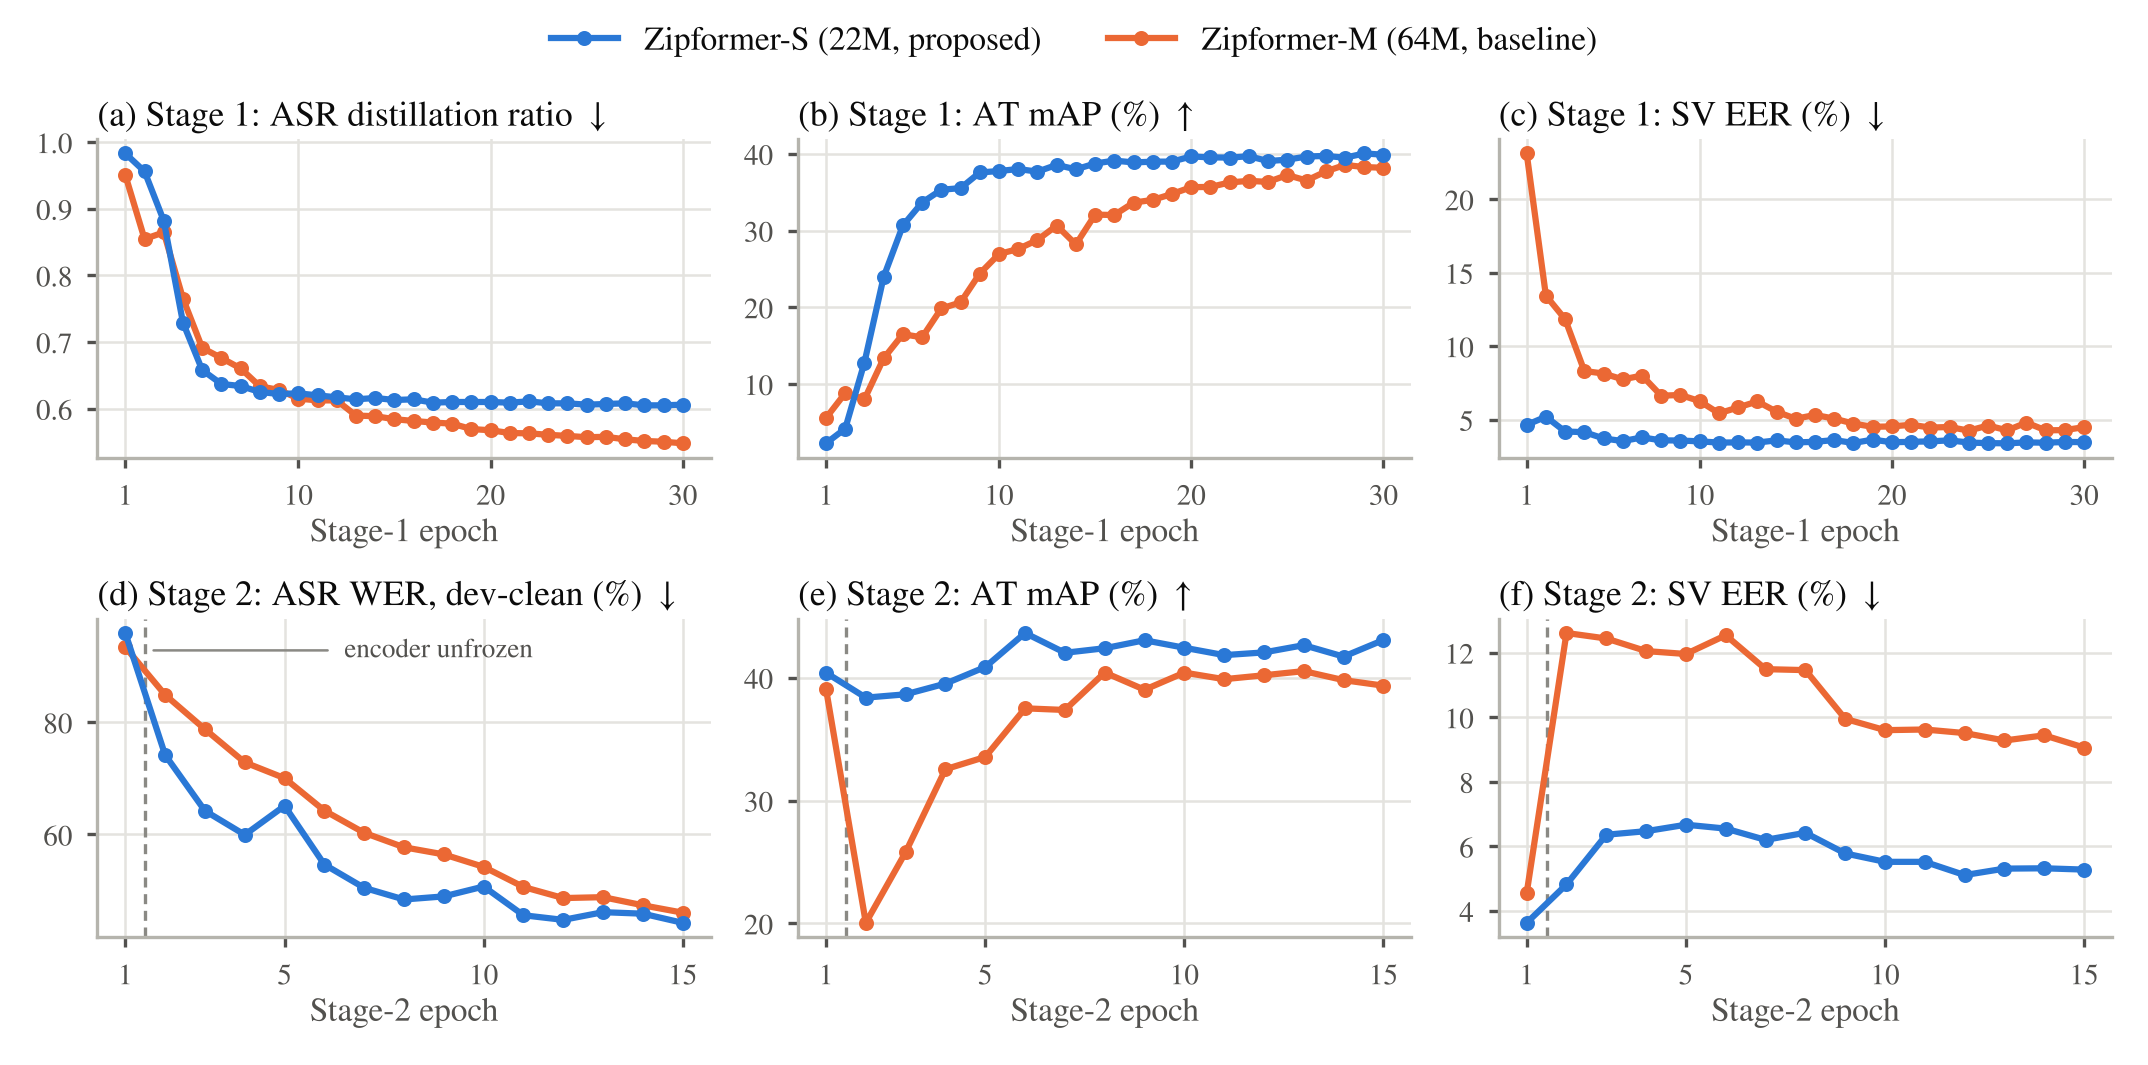
\includegraphics[width=\textwidth]{figures/fig_training_curves.png}
  \caption{Validation metrics after every epoch for Zipformer-S (22\,M, proposed) and Zipformer-M (64\,M, baseline).
  Top: Stage~1 (ASR distillation ratio, AT mAP, SV EER on the non-official validation speakers). Bottom: Stage~2
  (dev-clean WER with greedy CTC, FSD50K validation mAP, SV EER); the dashed line marks the end of the frozen-encoder
  warm-up.}
  \label{fig:curves}
\end{figure*}

\section{Results and Analysis}\label{sec:results}

\subsection{Baseline Results}
The 64\,M baseline reaches 45.08\% WER on test-clean (dev-clean 46.07\%, CER 15.29\%), 39.36\% mAP on FSD50K, and
8.44\% EER on VoxCeleb1-O. A pilot run on 10\,h of speech, 5,000 clips, and 60 speakers gave 78.80\%, 21.30\%, and
27.66\%; its 60 speakers were too few, as its speaker embeddings matched the teacher on training utterances (cosine
0.83) but not on held-out speakers (0.17). These are our own results; the numbers of Yang
\textit{et al.}~\cite{yang2025mt2kd}, obtained with far more data (960\,h of LibriSpeech, AudioSet, and VoxCeleb1 and 2)
and other teachers, are not directly comparable.

\subsection{Zipformer-S versus Zipformer-M}
Table~\ref{tab:s20} compares the proposed 22\,M student with the 64\,M baseline. Both were trained on the same data
with the same 30 + 15 epoch schedule and evaluated on the same official test sets.

\begin{table}[!htbp]
  \caption{Main results on the official test sets: Zipformer-S versus Zipformer-M (same data and schedule)}
  \label{tab:s20}
  \centering
  \footnotesize
  \setlength{\tabcolsep}{2.5pt}
  \begin{tabular}{L{1.95cm}ccccc}
    \toprule
    Model & Params & \shortstack{test-clean\\WER $\downarrow$} & \shortstack{FSD50K\\mAP $\uparrow$} & \shortstack{Vox1-O\\EER $\downarrow$} & \shortstack{CPU\\RTF $\downarrow$} \\
    \midrule
    Zipformer-M (baseline) & 64.35M & 45.08\% & 39.36\% & 8.44\% & 0.0360 \\
    \textbf{Zipformer-S (proposed)} & \textbf{22.44M} & \textbf{43.36\%} & \textbf{43.07\%} & \textbf{4.30\%} & \textbf{0.0246} \\
    \bottomrule
    \multicolumn{6}{L{8.2cm}}{\scriptsize Greedy CTC without an LM; mAP on the FSD50K validation split (200 classes); RTF for encoder + greedy CTC, 2 CPU threads, batch 1, fp32 (Section~\ref{sec:setup}).}
  \end{tabular}
\end{table}

The student is better than the baseline on all three tasks: 1.7 points lower WER on test-clean (dev-clean WER
44.26\% vs 46.07\%, CER 13.89\% vs 15.29\%), 3.7 points higher mAP, and about half the speaker-verification error (4.30\% vs 8.44\%). At the
same time it has 2.9$\times$ fewer parameters and runs 1.46$\times$ faster on the CPU. The speed gain is smaller than
the reduction in size because Zipformer-S only narrows stacks S3--S5, which run at the lowest frame rates, while
the front end and stacks S1, S2, and S6, where most of the computation happens, are identical in both models.

\subsection{Effect of Each Training Stage}
Table~\ref{tab:stages} tracks both encoders across the two stages, using the validation measurements available after
each stage.

\begin{table}[!htbp]
  \caption{Stage~1 versus Stage~2 (validation sets)}
  \label{tab:stages}
  \centering
  \footnotesize
  \setlength{\tabcolsep}{3pt}
  \begin{tabular}{L{1.75cm}L{1.35cm}L{1.35cm}L{1.55cm}L{1.55cm}}
    \toprule
    & \multicolumn{2}{c}{After Stage~1} & \multicolumn{2}{c}{After Stage~2} \\
    Metric & M (64M) & S (22M) & M (64M) & S (22M) \\
    \midrule
    ASR & ratio 0.548 & ratio 0.606 & WER 46.07\% & \textbf{WER 44.26\%} \\
    AT mAP & 38.18\% & \textbf{39.89\%} & 39.36\% & \textbf{43.07\%} \\
    SV EER (non-official) & 4.49\% & \textbf{3.47\%} & 9.06\% & \textbf{5.28\%} \\
    \bottomrule
  \end{tabular}
\end{table}

For ASR, the Stage-1 figure is the distillation ratio: the validation L1 loss divided by the L1 loss of a constant
prediction equal to the mean teacher feature, so 1.0 means no learning and lower is better. The SV figures are on the
non-official validation set of 40 held-out VoxCeleb1 development speakers. After Stage~1 the student is already better
on AT and SV but behind on the ASR distillation ratio; the narrower middle stacks reproduce the 2048-D WavLM features
less closely. Stage~2 closes this gap, and the student ends ahead on ASR as well.

For both encoders, supervised fine-tuning added a usable ASR output and raised AT mAP, but degraded speaker
verification. For Zipformer-M the SV EER doubled, from 4.49\% after Stage~1 to 9.06\% after Stage~2. The logs show
when this happened: SV EER was 4.55\% after the first Stage-2 epoch, while the encoder was still frozen, and rose to
12.6\% once the encoder was unfrozen, before settling at 9--12\%. AT showed a similar but temporary dip at the same
point (39.1\% to 20.1\%) and then recovered. Zipformer-S showed the same effect in a much milder form (3.47\% after
Stage~1 and 5.28\% after Stage~2). This is consistent with the observation in MT2KD that speaker information degrades
during joint fine-tuning, which the base work handled by freezing the SV parameters in Stage~2~\cite{yang2025mt2kd}.

\subsection{Equal-Training Comparison}
Fig.~\ref{fig:curves} shows the validation metrics of both encoders after every epoch of both stages.



In Stage~1 (Fig.~\ref{fig:curves}a--c) the student is ahead on AT and SV from the first epochs (after epoch 4:
mAP 23.96\% vs 13.35\%, EER 4.15\% vs 8.31\%), while on the ASR distillation ratio the two are level until about
epoch 10, after which the baseline keeps improving and the student levels off. In Stage~2 (Fig.~\ref{fig:curves}d--f) two effects stand out. First, the student learns faster: from the second epoch on it is ahead on every task (after epoch 5: WER 65.10\% vs 70.02\%, mAP 40.87\% vs 33.55\%, EER 6.67\% vs 11.96\%).
Second, it is far more stable when the encoder is unfrozen. Between epochs 1 and 2, the AT mAP of Zipformer-M fell
from 39.10\% to 20.05\% and its SV EER rose from 4.55\% to 12.61\%, whereas Zipformer-S moved only from 40.41\% to
38.38\% and from 3.63\% to 4.82\%. We attribute this mainly to the copy term of Eq.~(\ref{eq:ta2}), which keeps the
student's outputs close to those of the finished baseline while its encoder adapts. Part of the student's advantage
is therefore borrowed from the baseline, whose final model itself had 15 Stage-2 epochs; this is inherent to
teaching-assistant distillation, and the student cannot be trained without first training the baseline.

\subsection{Language-Model Decoding}
For the 64\,M baseline, the 3-gram language model lowered the dev-clean WER on 1,446 utterances of held-out speakers
from 46.33\% to 20.42\% (CER 15.42\% to 9.47\%), a relative reduction of 55.9\%, with $\alpha=0.7$ and $\beta=3.0$
tuned on the other speakers: much of the greedy-CTC error is spelling and word choice that word context can correct.
Table~\ref{tab:lm_both} applies the same decoder, language model, and tuning protocol to both encoders on test-clean.

\begin{table}[!htbp]
  \caption{Language-model decoding of both encoders on test-clean (same decoder, LM, and tuning protocol)}
  \label{tab:lm_both}
  \centering
  \footnotesize
  \setlength{\tabcolsep}{3pt}
  \begin{tabular}{L{2.0cm}L{1.5cm}L{1.9cm}L{1.6cm}}
    \toprule
    Model & Greedy WER $\downarrow$ & $+$ 3-gram LM WER $\downarrow$ & Relative reduction \\
    \midrule
    Zipformer-M (64M) & \ph{measured} & \ph{measured} & \ph{measured} \\
    Zipformer-S (22M) & \ph{measured} & \ph{measured} & \ph{measured} \\
    \bottomrule
  \end{tabular}
\end{table}

% ================================================================ VI. DISCUSSION
\section{Discussion}\label{sec:discussion}

\subsection{Limitations}
The training data are small (30\,h of speech, 15,000 clips, and 30,000 speaker utterances), which explains the high
greedy-CTC WER compared with systems trained on 960\,h. ASR uses character CTC rather than MT2KD's transducer, AT is
evaluated on the FSD50K validation split, and all results come from one run per model. Zipformer-S depends on a fully
trained Zipformer-M, so its total cost includes the baseline's, and the two encoders used different batch sizes (300
and 800\,s of audio). The language-model result is a separate decoding condition.

\subsection{Ethical Considerations}
Speaker embeddings are biometric data: their collection and use must respect licences, consent, and privacy, and
speaker verification should be deployed only for authorised uses. ReDimNet2-B6 was trained on VoxCeleb2 only, so it
shares no speakers with the VoxCeleb1 test set.

\subsection{Future Work}
The most direct next step is a \emph{task-conditioned Zipformer block}, motivated by the speaker-verification
degradation measured in Stage~2: the attention, convolution, and feed-forward modules inside each block stay shared
by all three tasks, while each task receives a few task-specific parameters within the block, namely its own bypass
gates (how strongly each block transforms its features), BiasNorm scales, and attention-head weights. This adds well
under 1\% of parameters, can be initialised from the trained shared model, and lets each task use the shared blocks
differently. Further steps are to train on the full LibriSpeech, FSD50K, and VoxCeleb corpora, to evaluate AT on the
official FSD50K evaluation set, to repeat the comparison with several random seeds, and to measure INT8 quantisation
for faster CPU inference.

% ================================================================ VII. CONCLUSION
\section{Conclusion}\label{sec:conclusion}
This paper presented \method{}, a multi-task audio framework in which one encoder performs speech recognition, audio
tagging, and speaker verification. Following the two-stage MT2KD recipe, we replaced the original teachers with
WavLM-Large, SSLAM, and ReDimNet2-B6, which cut the teacher parameters by about 44\% while each replacement measured
better than the model it replaced. A 64\,M Zipformer-M baseline trained this way reaches 45.08\% WER on LibriSpeech
test-clean, 39.36\% mAP on FSD50K, and 8.44\% EER on VoxCeleb1-O. Using it as a frozen teaching assistant and copying
its shared stacks, a 22\,M Zipformer-S trained on the same data and schedule reaches 43.36\%, 43.07\%, and 4.30\%,
respectively, while being 2.9$\times$ smaller and 1.46$\times$ faster on a CPU and much more stable during
fine-tuning. A 3-gram language model lowers the dev-clean WER of the baseline from 46.33\% to 20.42\%. The stage-wise
analysis shows that protecting the speaker branch during fine-tuning is the most promising route to further gains.

% ================================================================ BACK MATTER
\section*{Data and Code Availability}
LibriSpeech, FSD50K, and VoxCeleb1 are publicly available under their respective terms, and the original datasets are
not redistributed. Code, configurations, and the trained models are available from the authors on reasonable request.

% References are inline (IEEE style, numbered in order of first citation).
\begin{thebibliography}{99}

\bibitem{yang2025mt2kd}
X.~Yang, Q.~Li, C.~Zhang, and P.~C. Woodland, ``MT2KD: Toward a general-purpose encoder for speech, speaker, and audio events,'' \emph{IEEE Trans. Audio, Speech, Lang. Process.}, vol.~33, pp.~3454--3464, 2025.

\bibitem{graves2006ctc}
A.~Graves, S.~Fern\'andez, F.~Gomez, and J.~Schmidhuber, ``Connectionist temporal classification: Labelling unsegmented sequence data with recurrent neural networks,'' in \emph{Proc. ICML}, 2006, pp.~369--376.

\bibitem{graves2012transducer}
A.~Graves, ``Sequence transduction with recurrent neural networks,'' in \emph{Proc. ICML Workshop on Representation Learning}, 2012.

\bibitem{radford2023whisper}
A.~Radford, J.~W. Kim, T.~Xu, G.~Brockman, C.~McLeavey, and I.~Sutskever, ``Robust speech recognition via large-scale weak supervision,'' in \emph{Proc. ICML}, 2023, pp.~28492--28518.

\bibitem{choi2016tagging}
K.~Choi, G.~Fazekas, and M.~Sandler, ``Automatic tagging using deep convolutional neural networks,'' in \emph{Proc. ISMIR}, 2016, pp.~805--811.

\bibitem{kong2020panns}
Q.~Kong \emph{et al.}, ``PANNs: Large-scale pretrained audio neural networks for audio pattern recognition,'' \emph{IEEE/ACM Trans. Audio, Speech, Lang. Process.}, vol.~28, pp.~2880--2894, 2020.

\bibitem{gong2021ast}
Y.~Gong, Y.-A. Chung, and J.~Glass, ``AST: Audio spectrogram transformer,'' in \emph{Proc. Interspeech}, 2021, pp.~571--575.

\bibitem{chen2023beats}
S.~Chen \emph{et al.}, ``BEATs: Audio pre-training with acoustic tokenizers,'' in \emph{Proc. ICML}, 2023, pp.~5178--5193.

\bibitem{snyder2019xvector}
D.~Snyder \emph{et al.}, ``Speaker recognition for multi-speaker conversations using X-vectors,'' in \emph{Proc. ICASSP}, 2019, pp.~5796--5800.

\bibitem{desplanques2020ecapa}
B.~Desplanques, J.~Thienpondt, and K.~Demuynck, ``ECAPA-TDNN: Emphasized channel attention, propagation and aggregation in TDNN based speaker verification,'' in \emph{Proc. Interspeech}, 2020, pp.~3830--3834.

\bibitem{tang2016multitask}
Z.~Tang, L.~Li, and D.~Wang, ``Multi-task recurrent model for speech and speaker recognition,'' in \emph{Proc. APSIPA ASC}, 2016, pp.~1--4.

\bibitem{pironkov2016overview}
G.~Pironkov, S.~Dupont, and T.~Dutoit, ``Multi-task learning for speech recognition: An overview,'' in \emph{Proc. ESANN}, 2016, pp.~189--194.

\bibitem{elizalde2024clap}
B.~Elizalde, S.~Deshmukh, and H.~Wang, ``Natural language supervision for general-purpose audio representations,'' in \emph{Proc. ICASSP}, 2024, pp.~336--340.

\bibitem{hsu2021hubert}
W.-N. Hsu \emph{et al.}, ``HuBERT: Self-supervised speech representation learning by masked prediction of hidden units,'' \emph{IEEE/ACM Trans. Audio, Speech, Lang. Process.}, vol.~29, pp.~3451--3460, 2021.

\bibitem{chen2022wavlm}
S.~Chen \emph{et al.}, ``WavLM: Large-scale self-supervised pre-training for full stack speech processing,'' \emph{IEEE J. Sel. Topics Signal Process.}, vol.~16, no.~6, pp.~1505--1518, Oct. 2022.

\bibitem{yang2021superb}
S.-w. Yang \emph{et al.}, ``SUPERB: Speech processing universal performance benchmark,'' in \emph{Proc. Interspeech}, 2021, pp.~1194--1198.

\bibitem{gong2023whisperat}
Y.~Gong, S.~Khurana, L.~Karlinsky, and J.~Glass, ``Whisper-AT: Noise-robust automatic speech recognizers are also strong general audio event taggers,'' in \emph{Proc. Interspeech}, 2023, pp.~2798--2802.

\bibitem{hinton2014distilling}
G.~Hinton, O.~Vinyals, and J.~Dean, ``Distilling the knowledge in a neural network,'' in \emph{Proc. NIPS Deep Learning Workshop}, 2014.

\bibitem{li2014smalldnn}
J.~Li, R.~Zhao, J.-T. Huang, and Y.~Gong, ``Learning small-size DNN with output-distribution-based criteria,'' in \emph{Proc. Interspeech}, 2014, pp.~1910--1914.

\bibitem{beyer2022patient}
L.~Beyer \emph{et al.}, ``Knowledge distillation: A good teacher is patient and consistent,'' in \emph{Proc. CVPR}, 2022, pp.~10925--10934.

\bibitem{mirzadeh2020takd}
S.~I. Mirzadeh, M.~Farajtabar, A.~Li, N.~Levine, A.~Matsukawa, and H.~Ghasemzadeh, ``Improved knowledge distillation via teacher assistant,'' in \emph{Proc. AAAI}, 2020, pp.~5191--5198.

\bibitem{takashima2018ctckd}
R.~Takashima, S.~Li, and H.~Kawai, ``An investigation of a knowledge distillation method for CTC acoustic models,'' in \emph{Proc. ICASSP}, 2018, pp.~5809--5813.

\bibitem{yang2022transducerkd}
X.~Yang, Q.~Li, and P.~C. Woodland, ``Knowledge distillation for neural transducers from large self-supervised pre-trained models,'' in \emph{Proc. ICASSP}, 2022, pp.~8527--8531.

\bibitem{gandhi2023distilwhisper}
S.~Gandhi, P.~von Platen, and A.~M. Rush, ``Distil-Whisper: Robust knowledge distillation via large-scale pseudo labelling,'' 2023, arXiv:2311.00430.

\bibitem{schmid2023efficientat}
F.~Schmid, K.~Koutini, and G.~Widmer, ``Efficient large-scale audio tagging via transformer-to-CNN knowledge distillation,'' in \emph{Proc. ICASSP}, 2023.

\bibitem{dinkel2024ced}
H.~Dinkel, Y.~Wang, Z.~Yan, J.~Zhang, and Y.~Wang, ``CED: Consistent ensemble distillation for audio tagging,'' in \emph{Proc. ICASSP}, 2024, pp.~291--295.

\bibitem{wang2019speakerkd}
S.~Wang, Y.~Yang, T.~Wang, Y.~Qian, and K.~Yu, ``Knowledge distillation for small foot-print deep speaker embedding,'' in \emph{Proc. ICASSP}, 2019, pp.~6021--6025.

\bibitem{huang2023ensemblekd}
K.-P. Huang \emph{et al.}, ``Ensemble knowledge distillation of self-supervised speech models,'' in \emph{Proc. ICASSP}, 2023.

\bibitem{yang2023multifoundation}
X.~Yang, Q.~Li, C.~Zhang, and P.~C. Woodland, ``Knowledge distillation from multiple foundation models for end-to-end speech recognition,'' 2023, arXiv:2303.10917.

\bibitem{ranzinger2024amradio}
M.~Ranzinger, G.~Heinrich, J.~Kautz, and P.~Molchanov, ``AM-RADIO: Agglomerative vision foundation model---Reduce all domains into one,'' in \emph{Proc. CVPR}, 2024, pp.~12490--12500.

\bibitem{yao2024zipformer}
Z.~Yao \emph{et al.}, ``Zipformer: A faster and better encoder for automatic speech recognition,'' in \emph{Proc. ICLR}, 2024.

\bibitem{sslam}
T.~Alex, S.~Atito, A.~Mustafa, M.~Awais, and P.~J.~B. Jackson, ``SSLAM: Enhancing self-supervised models with audio mixtures for polyphonic soundscapes,'' in \emph{Proc. ICLR}, 2025.

\bibitem{redimnet2}
I.~Yakovlev and A.~Okhotnikov, ``ReDimNet2: Scaling speaker verification via time-pooled dimension reshaping,'' in \emph{Proc. Interspeech}, 2026, arXiv:2603.11841.

\bibitem{sanh2019distilbert}
V.~Sanh, L.~Debut, J.~Chaumond, and T.~Wolf, ``DistilBERT, a distilled version of BERT: Smaller, faster, cheaper and lighter,'' in \emph{Proc. NeurIPS Workshop on Energy Efficient Machine Learning and Cognitive Computing}, 2019, arXiv:1910.01108.

\bibitem{howard2018ulmfit}
J.~Howard and S.~Ruder, ``Universal language model fine-tuning for text classification,'' in \emph{Proc. ACL}, 2018, pp.~328--339.

\bibitem{panayotov2015librispeech}
V.~Panayotov, G.~Chen, D.~Povey, and S.~Khudanpur, ``Librispeech: An ASR corpus based on public domain audio books,'' in \emph{Proc. ICASSP}, 2015, pp.~5206--5210.

\bibitem{fonseca2022fsd50k}
E.~Fonseca, X.~Favory, J.~Pons, F.~Font, and X.~Serra, ``FSD50K: An open dataset of human-labeled sound events,'' \emph{IEEE/ACM Trans. Audio, Speech, Lang. Process.}, vol.~30, pp.~829--852, 2022.

\bibitem{nagrani2017voxceleb}
A.~Nagrani, J.~S. Chung, and A.~Zisserman, ``VoxCeleb: A large-scale speaker identification dataset,'' in \emph{Proc. Interspeech}, 2017, pp.~2616--2620.

\bibitem{gemmeke2017audioset}
J.~F. Gemmeke \emph{et al.}, ``Audio Set: An ontology and human-labeled dataset for audio events,'' in \emph{Proc. ICASSP}, 2017, pp.~776--780.

\end{thebibliography}

\end{document}
